\documentclass{llncs}

\usepackage{floatrow}
\usepackage[utf8]{inputenc}
\usepackage{url}
%% This was made necessary to break` long URLs, no other system I tried worked and a few URLs still fail; see http://tex.stackexchange.com/a/10419/60582 
\makeatletter
\g@addto@macro{\UrlBreaks}{\UrlOrds}
\makeatother
\usepackage{graphicx}
\graphicspath{{./images/}}

\title{Using hybrid human-machine workflows to create geospatial data}

\author{AUTHOR 1\inst{1}, AUTHOR 2\inst{1} \and AUTHOR 3\inst{2}}
\institute{INSTITUTE 1 \email{EMAIL FOR AUTHOR 1} \and INSTITUTE 2}

\date{December 2015}

\begin{document}

\maketitle

\begin{abstract}
As more open data is published by governments and organisations, the task of creating new data evolves from being a ground-up process - where data is collected and shaped from scratch - to an enhancement process, where pre-existing sources and original additions merge into new, valuable data products. 

Machine learning, computer vision and automation in general can't (yet?) address all challenges in this area, and available data, computation and original contributions by human participants - e.g. through crowdsourcing - need integration and enabling each other through hybrid human-machine workflows. 

In this paper we present an experimental platform that implements this model, aimed specifically at the creation of geospatial data. The platform is then applied to a real world use case: the creation of "OLAF", an open dataset of all valid UK addresses, starting from available open data and augmenting it through computational inference and microtask crowdsourcing. Experimental evaluation show the feasibility and effectiveness of the approach.
\end{abstract}

\begin{keywords}
Crowdsourcing, Geographic Information, hybrid human-machine systems, open data 
\end{keywords}

\begin{itemize}
    \item MAX 18 PAGES
    \item OPEN POINTS
        \begin{itemize}
            \item XXX
        \end{itemize}
    \item WEAKNESSES 
        \begin{itemize}
            \item STRONG FOCUS ON USE CASE, POOR GENERALISATION, BUT IS IT NECESSARY?, GIVEN THE CONFERENCE'S EXPLICIT INTEREST IN "Use cases and experiences with human computing and crowdsourcing applications" \url{http://icwe2016.inf.usi.ch/topics#crowd}
        \end{itemize}
\end{itemize}

\section{Introduction}

Geospatial data is a critical component of many applications. Its value is universally recognised to be instrumental to development [SOME REFERENCE], yet not all of it is readily available, and, when it is, its use is associated with high costs or restrictive licensing. 

The availability of geospatial data under an open licensing in particular is not only limited, but the effort national mapping and cadastre agencies (NMCAs) worldwide put into producing and updating cartography and their other assets for the public good has been in decline for several decades \cite{ESTES:1994vz}. In the U.S., for example, the Geological Survey (USGS) no longer attempts to update its maps on a regular basis and the National Research Council promotes a vision in which the creation and curation geospatial data is no longer centralised but rather shared and consolidated from many governmental and private sector sources \cite{Committee:1993vp}.

In this document, [DON'T LIKE THIS EXPRESSION we look at one possible solution to these problems] and propose a platform to create and curate geospatial data that integrates pre-existing open data, computation and original contributions by human participants - typically through crowdsourcing - in hybrid human-machine workflows. The platform can be configured to produce different kinds of data, support different types of crowdsourcing models (tasks, participation, rewards to participants etc) and is made available as open source.

We then focus on a specific use case: the creation of the list of all valid addresses in the UK, or the "Open Legal Address File" ("OLAF"), which has received a lot of attention in the country as it a great example of simple, though critical, geographic data that is unfortunately available only as a commercial product. We use the platform to implement one of the possible workflows to create parts of OLAF, and evaluate its performance. 

We believe this could be a useful tool for geospatial researchers and practitioners interested in systematically using crowdsourcing in their daily work.

\section{Background and related work}

\subsection{Crowdsourcing geospatial information}

Geographical Information Systems (GIS) are systems designed to capture, manipulate, analyse and visualise geographical data. 

Crowdsourcing geographical data was made possible in the early 2000's by the availability of GIS to the wider public. As web technology matured, publicly available, web-based GIS systems emerged including OpenStreetMap\footnote{Created in 2004, see \url{https://www.openstreetmap.org}.} (OSM), Google Maps\footnote{Launched in 2005, see \url{https://www.google.com/maps}. Google Earth is actually precedent to Google Maps and was launched in 2001, but at the time it was available as a downloadable desktop application only.} and Wikimapia\footnote{Created in 2006, see \url{http://wikimapia.org/}.}. In what was by some called "the democratisation of GIS" \cite{Butler:2006fe} laypeople could for the first time contribute to the systems, augmenting pre-existing data and creating new. This was around the same time the term "crowdsourcing" was used first\footnote{J. Howe, "The Rise of Crowdsourcing" Wired, 01-Jun-2006.}.

Crowdsourcing geospatial data became the subject of extensive research. Because of the origins of the phenomenon, volunteered rather than paid participation to the systems was studied in particular, to the point of defining the discipline itself. In 2007 Michael F. Goodchild coined the term "Volunteered Geographic Information" (Volunteered GI, or VGI) \cite{Goodchild:2007vt} and examined it as a new form of citizen science. Goodchild also was among the first to make the hypothesis that relying on the crowd could be more cost-effective at maintaining geospatial data than any of the traditional ways.

\subsection{Challenges of crowdsourcing geospatial data}
\label{challenges-of-crowdsourcing-geospatial-data}

There are a number of recognised challenges in crowdsourcing geospatial data. The most relevant to our research are summarised here.

\textbf{Contributor credibility} The trustworthiness and expertise of a contributor defines her "credibility". In cases where crowdsourced GIS systems are designed to be accessible to the layperson and do not require specific expertise, the only credibility variable remains trustworthiness, which depends on the contributor's motivation, which in turn "suggests greater or less potential for bias and deception" \cite{Flanagin:2008ck}. Gatekeeping and quality control are practices used to assure contributor credibility. 

In our research paid crowdsourcing was used to cancel out bias.

\textbf{Data reliability} Even assuming that the contributors are individually credible, it is necessary to assess the quality of the system's overall output. 

The reliability of mainstreams VGI systems was assessed for example by Haklay in \cite{Haklay:2010vs}, who performed a comparative study of data offered by OSM and the British NMCA Ordnance Survey (OS). In 2008, only a few years after OSM was started, OSM offered a "reasonable accuracy" of about 6 meters and an overlap of up to 100\% of roads in OS' data. 

Further research in \cite{Haklay:2010wf} suggests that the volume of volunteers involved in a project - even when working without a central coordination - can be considered as an intrinsic quality assurance measure.

In our research, using paid crowdsourcing gave us more direct control over the volume of contributors we could engage on creating or validating the data and enabled us to use more robust statistical tools.

\textbf{Data completeness} Volunteered GI has a completeness issue, in the words of OSM creator Steve Coast: "Nobody wants to do council estates"\footnote{"The GISPro Interview with OSM founder Steve Coast" GIS Professional, no. 18, 2007.}. Loose organisation of the contributors and a range of socioeconomic barriers \cite{Haklay:2010vs} may hinder achievement of sufficient coverage of those geographical areas volunteers are not motivated to contribute about.

Moreover, some applications may require the data to be produced within a given timeframe, not compatible with volunteer best effort, something that could be better controlled using paid crowdsourcing.

\textbf{Domain knowledge} Contributors to GI crowdsourcing projects need a sufficient understanding of the concepts that define the domain, such as what a road is, what a building etc. \cite{Ballatore:2015kg}. 

In our work we tried minimising this requirement, by simplifying the contributor task down to making simple observations from imagery of the surveyed locations.

\subsection{Open data and open Geographic Information}
\label{open-data-and-gi}

Because research has focussed on systems that leverage volunteer contribution and are designed for the pubic good, GI is often implicitly associated to open data: "data that anyone can access, use and share"\footnote{\url{http://theodi.org/faq}.}. 

Government-funded NMCAs are natural owners of geospatial data and are commonly expected to release it in the open for the public good. In Great Britain, for example, since 2015 the local NMCA Ordnance Survey (OS) has opened a substantial volume of data that was previously available to the public as commercial products only, including products such as "Open Names" - a place-name index - and "Open Roads" - the generalised geometry and network connectivity of the road network - which we used in our platform as primary data sources.
	
The availability of such high quality and authoritative sources becomes a substantial enabler for the creation of new, original geospatial data and augmenting what is already available.

All useful and needed geospatial data is not always made available in the open, though. Demand for open data can be suppressed, for example, due to failure in recognising open data-enabled business models, restrictive legislative and patent systems, or charging for access\footnote{N. Shadbolt, "A Cornerstone for Open Data: The Postcode Address File" Apr-2013. Online. Available: \url{http://theodi.org/blog/cornerstone-open-data-postcode-address-file}. Accessed: 09-May-2015.}. The OLAF problem, described later in this document, is an example of this.
	
\subsection{The Open Legal Address File (OLAF)}
\label{subs:the-problem-of-creating-an-olaf}

The main use case for our research is creating an Open Legal Address File\footnote{See \url{https://github.com/Digital-Contraptions-Imaginarium/OLAF-yr2_lab/blob/gh-pages/docs/README.md#legal-address-files} for an explanation of the "legal address" term.} for the UK: a dataset that is functionally equivalent, for example, to Royal Mail's "Postcode Address File" ("PAF"\footnote{PAF is a registered trademark by Royal Mail plc. For convenience we won't show the registered trademark sign "\textregistered" in this document every time we refer to it.}). 

\textbf{The Postcode Address File} PAF is a commercial dataset that lists all known valid addresses and postcodes for the UK and was created by the previously state-owned mail delivery services company over many years of operations.

PAF is by law\footnote{See the Postal Service Act 2000, part VII, article 116, available at \url{http://www.legislation.gov.uk/ukpga/2000/26/contents}.} the ownership of Royal Mail, to be made available on "reasonable terms" to "any person who wishes to use it". This, however, never translated into making the data open. The dataset is available from Royal Mail and its resellers as a commercial product, and was privatised together with Royal Mail and its other assets in October 2013\footnote{Royal Mail is currently a public limited company with only a 30\% of shares controlled by the Government. The Postal Services Act 2011, available at \url{http://www.legislation.gov.uk/ukpga/2011/5/contents}, plans to reduce the Government control down to 10\%.}. OLAF aims to fill the gap left in the UK open geospatial data offering. 

\textbf{The OLAF data model} OLAF is a flat list of valid UK addresses. Without going into the detail of official British Standard BS7666\footnote{See \url{http://shop.bsigroup.com/ProductDetail/?pid=000000000030127201}.}, a practical operational definition of a "valid UK address" would be {\it the set of unambiguous information needed to instruct any delivery service operator to deliver a piece of mail at a given public address (a private house, a commercial establishment etc.), from a consumer perspective}. 

An address is characterised by the following properties:

\begin{itemize}
    \item A "primary addressable object name" (PAON), e.g. "10". The PAON identifies one property.
    \item A "secondary addressable object name" (SAON), e.g. "Flat 2". The SAON identifies a part of a property and is optional.
    \item A street name\footnote{For simplicity, note that the terms "place", "road" or "street" are used interchangeably here and in the rest of this document, as they are equivalent from an OLAF perspective. The "street name" in the model above, for example, may be the name of a square, etc.}, e.g. "Downing Street".
    \item A town name, e.g. "London".
    \item A UK postcode, e.g. "SW1A 2AA".
\end{itemize}

\section{Platform}

\subsection{Overview}

This section describes the general-purpose platform that was designed and built for the creation and curation of geospatial data, enabled by hybrid human-machine workflows. 

The general workflow model that was used as reference is shown in ****.

[FIGURE]

From the platform owner point of view, the system is made of:

\begin{enumerate}
    \item A set of tools to ingest the primary data sources into a reference database.
    \item A set of tools to process the ingested data and derive new / enhanced data computationally, e.g. through statistical inference.
    \item A set of templates to configure the crowdsourcing platform of choice - e.g. Amazon Mechanical Turk or CrowdFlower - and set up the interface the participants use to contribute.
    \item A set of tools to iteratively (i) identify what the highest priority gaps in the reference and derived data are, (ii) load data into the crowdsourcing platform accordingly, to enable the collection of what is missing and (iii) evaluate the crowd's output, until a stop condition is verified, e.g. the data was successfully collected and at the target level of quality, or, in the case of paid crowdsourcing all budget has been spent.
    \item A set of tools to consolidate the original, derived and crowdsourced data in one consistent dataset.
\end{enumerate}

From the participant point of view, the solution presents itself simply as a task hosted on their crowdsourcing platform of choice. The task web page offers interactive maps and a panoramic views of one or more locations to survey, and a form the participant will use to submit her observations, as shown in \ref{fig:virtual-survey-tool-01}. 

At the top of the page, for contributors who are new to the task, instructions are given, possibly enhanced by a video used to illustrate the interactive features of the map and panoramic view, as in \ref{fig:virtual-survey-tool-02}.

\begin{figure}[!h]
    \begin{floatrow}
        \ffigbox{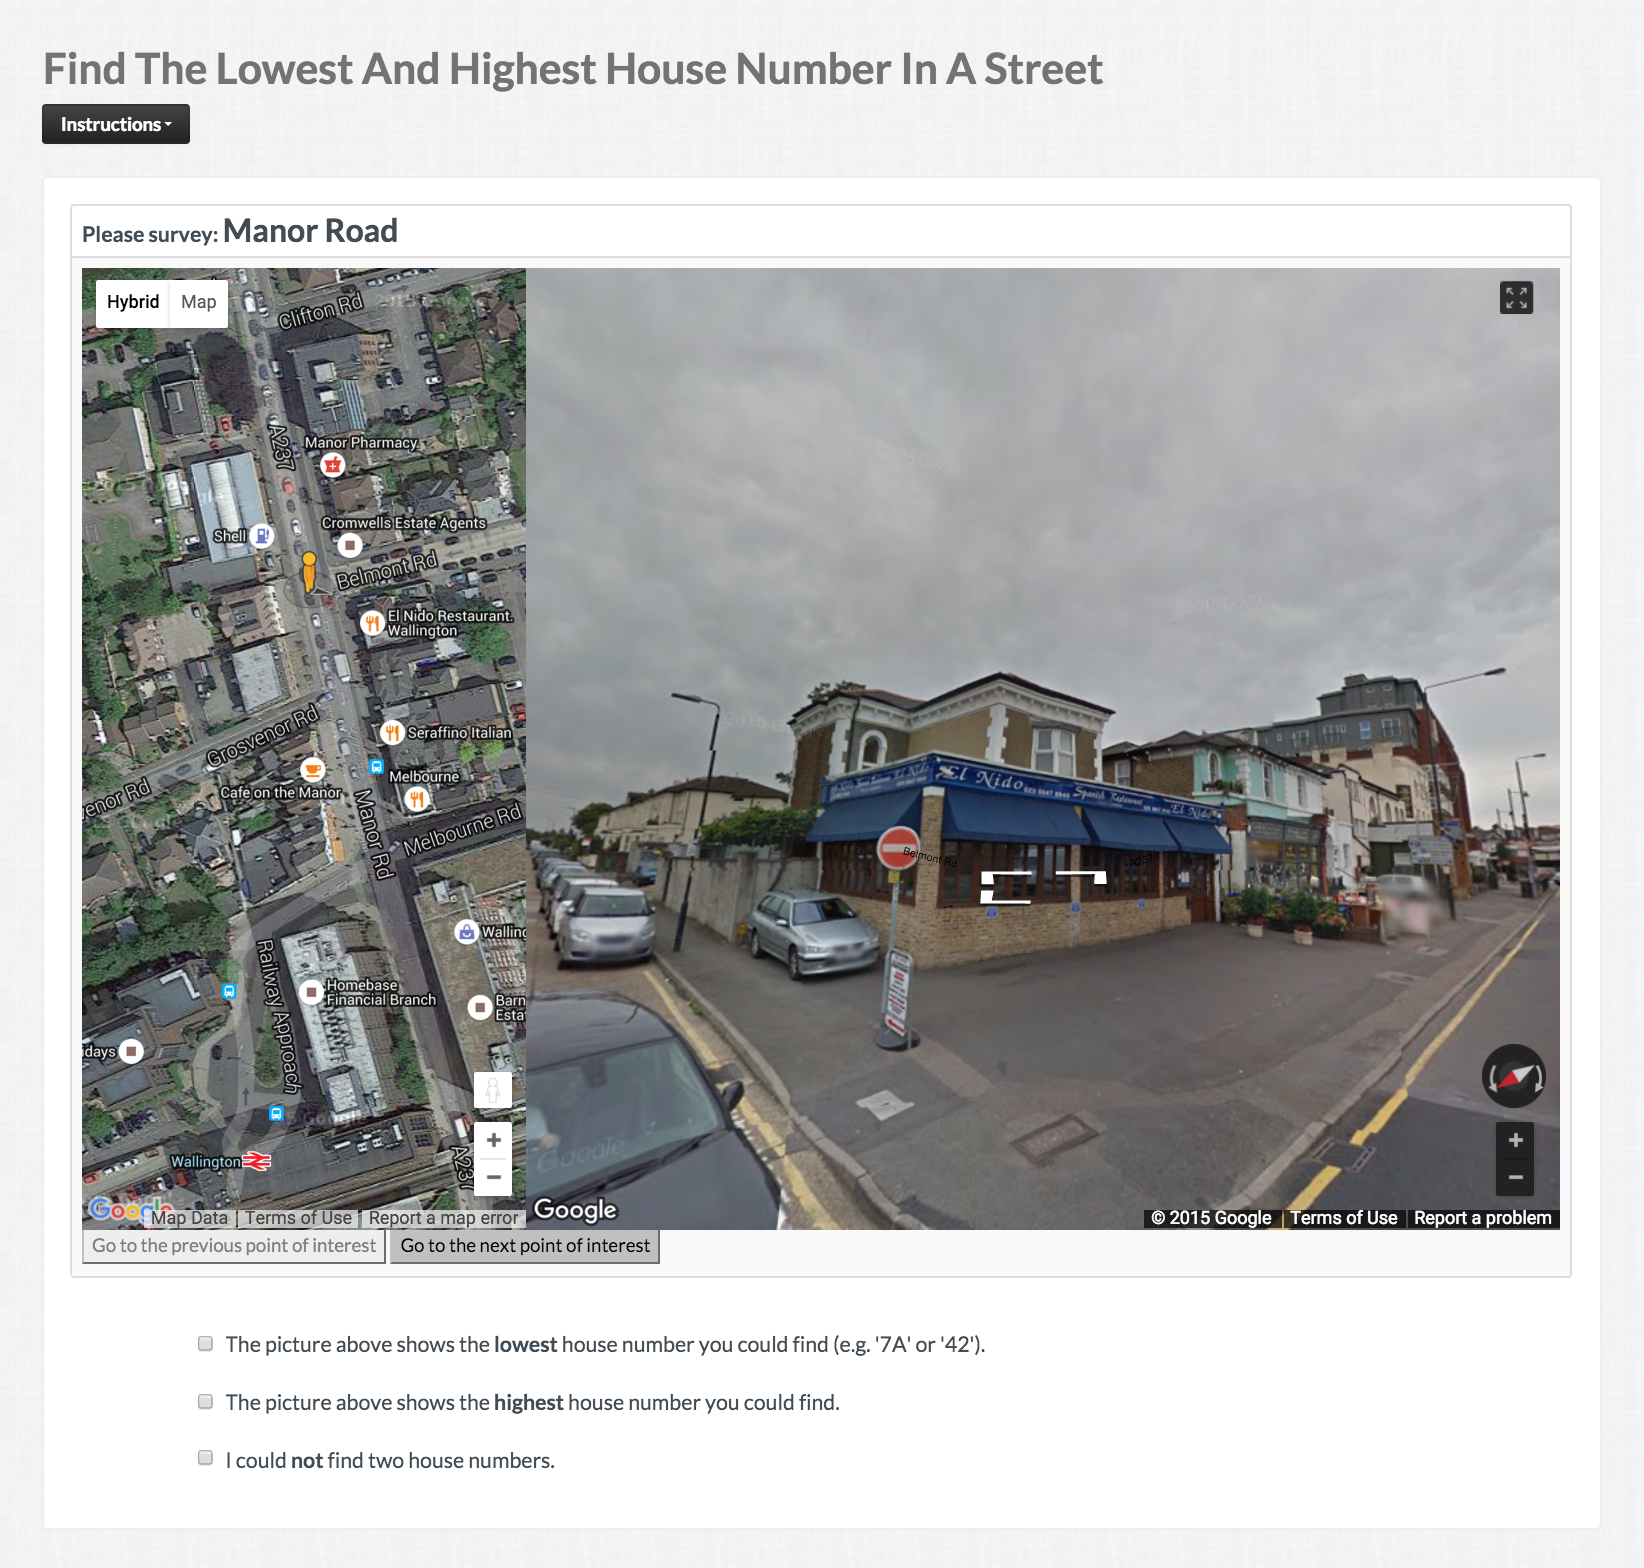
\includegraphics[width=0.45\textwidth]{virtual-survey-tool-01.png}}{\caption{The task section of the web page, offering the Google Maps and Street View panes and the form participants use to submit their observation.}\label{fig:results-highest-not-found}}
        \ffigbox{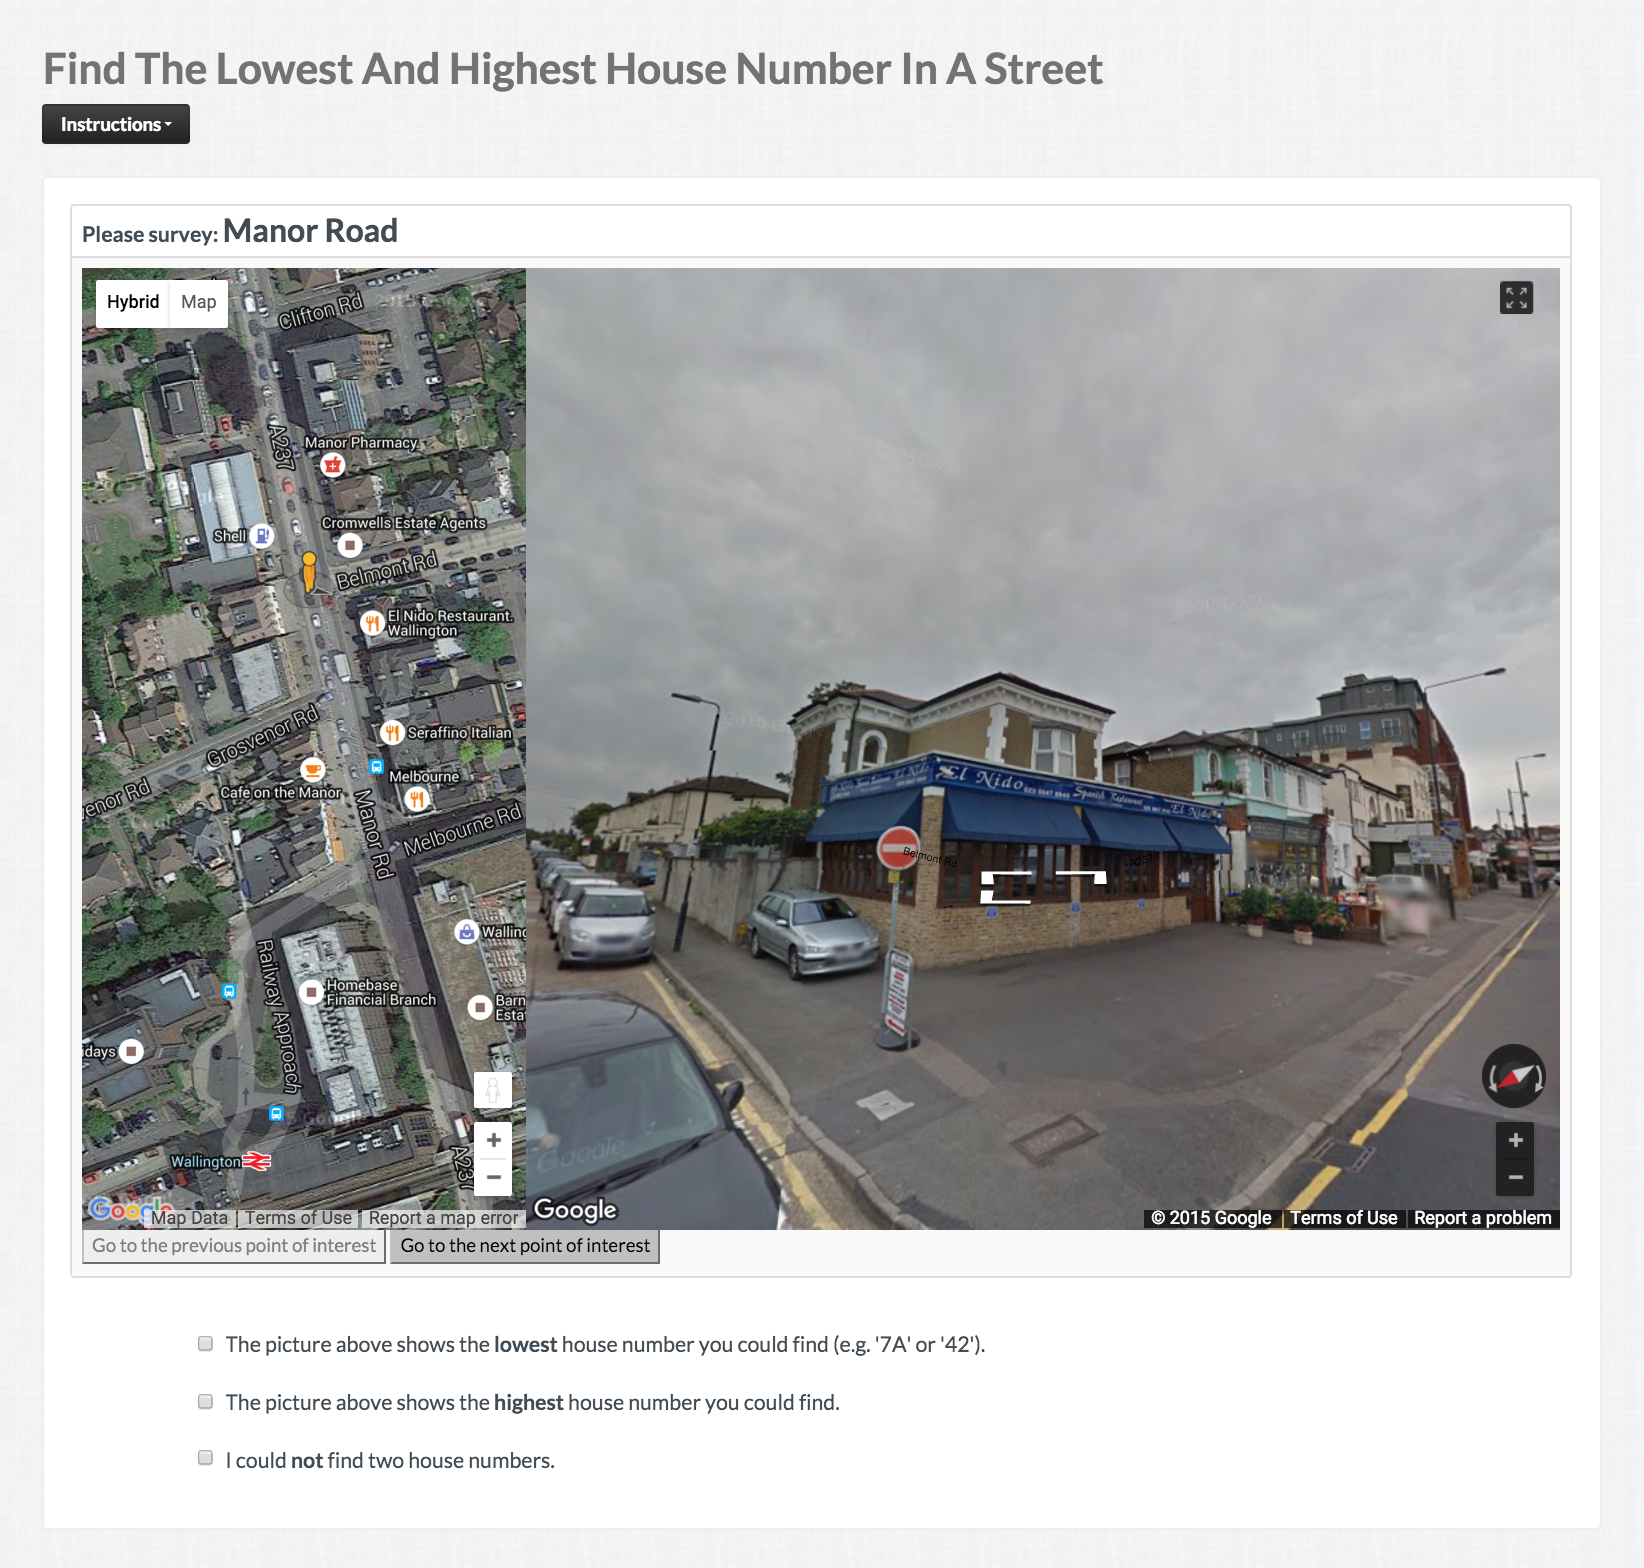
\includegraphics[width=0.45\textwidth]{virtual-survey-tool-01.png}}{\caption{The instruction section of the web page, embedding a video with the instructions.}\label{fig:virtual-survey-tool-02}}
   \end{floatrow}
\end{figure}

\subsection{Overall design principles}

In designing the platform, design principles below were used as guidance:

\textbf{Support to human-machine workflows} The opportunity to exploit hybrid human-machine workflows was a key assumption in our research. The solution was required to automate as much as possible of the data creation / curation process while effectively integrating human components, from the crowdsourcing of part of the data to the administration of the process itself.

\textbf{Data re-use} Making the best possible use of pre-existing, reliable data was a key design driver, in particular to take advantage of the substantial volume of open data published in the UK over the last two-three years, and expecting a similar trend to be observable in many other countries in the upcoming years.

\textbf{Open source software} It was assumed that most original components required by the solution could be built using open source software only, also to preserve any available budget for the compensation of paid contributors to the crowdsourcing campaigns.

\textbf{Scalability and high availability} The solution was designed to be highly scalable and available - well beyond the needs of the experiments described later in this document - and suitable for real-world deployment.

\textbf{Versatility} The solution needed being versatile and suitable to support different workflows, input data sources and target output datasets. Despite the extensive literature, crowdsourcing in particular is still more of a craft than science and no design formula can assure success without experimentation. The design of the solution needed to support different forms of crowdsourcing across its many dimensions: paid contributors vs volunteers, results aggregation, quality assessment etc.

\subsection{Crowdsourcing component design principles}

The following is a high level description of the crowdsourcing component of the platform according to the dimensions presented in \cite{Wearethedata:2015uo}. The description is independent of the specific objective of the system. 

A general observation is that the crowdsourcing element was intentionally designed to explore characteristics that are far from what has been already extensively explored in VGI literature, particularly thanks to the opportunity to study the OpenStreetMap case. The hypothesis and ambition is that the finding of the research can be complementary to what can be achieved with VGI and enrich the set of tools available to the system designer.

\textbf{What is outsourced} The objective of the outsourcing activity is the production of original geospatial data or the correction / validation of pre-existing data, wherever the activity can be only performed by human agents. 

We use the term "geospatial data" in its wider connotation: data that relates to or is associated with a particular location. It can be about the geographic characteristics of a place (e.g. the topology of a street network), but also about facts associated to that place (e.g. how many trees in that street).

The activity typically translates into surveying the locations or examining imagery thereof and record observations (e.g. "how many trees can be seen from longitude x and latitude y?"), or, alternatively, amend some previous recording of the same (e.g. "can you confirm that there is a hospital in Vicarage Rd, Watford, Hertfordshire?"). 

To avoid the physical survey of the locations, participants examine publicly available imagery of the location. This is not uncommon, e.g. the OpenStreetMap website uses aerial imagery sourced from Microsoft Bing to let its contributors edit the topology of the streets\footnote{See \url{https://www.openstreetmap.org/edit}.}. The cost effectiveness of humans observers is expected to outperform machine learning, computer vision and automation in general for a few more years, particularly in observing imagery that are ambiguous [IT WOULD BE NICE TO QUOTE SOMEONE HERE].

\textbf{Who is the crowd} No specialised knowledge or skills are required, nor a connection to the places being surveyed. In VGI, though, contributors are often associated to the locations they work on, as it is both a driver for their motivation and direct knowledge of the place is occasionally necessary to assure the completeness of the data. The function of buildings or the location of mailboxes, for example, can't be inferred from observing OpenStreetMap's aerial imagery. Moreover, the first survey of new locations, e.g. new developments before they are visible on aerial imagery, are often made using specialised equipment, e.g. to record GPS tracks\footnote{E.g. the OpenStreetMap project advises against using conventional mobile phone GPS functionality, as it can be very difficult to work out the technical accuracy of a track. See \url{http://wiki.openstreetmap.org/wiki/Recording_GPS_tracks}.}.

The crowdsourcing task design intends to assure the contributors detachment from the locations.

\textbf{How are the task outsourced} Again, to explore different formulae than what is common in VGI, the crowdsourcing component focus is on implementing micro rather than macro tasks, and, definitely, microtasks cannot be burdened with the overhead typical of surveying in the real world, like planning a journey and travelling to the location and back, use equipment etc. 

Wherever possible, one's contribution is limited to max few minutes of work at the computer, the shorter the time required the better. Ideal tasks are closed- rather than open-ended and require no particular thought or focus. The participant has no visibility of the workflow she is part of: the volume of effort spent in preparing the data, aggregating the responses, assessing their accuracy etc. 

\textbf{Why do people contribute} In VGI, crowds are made of intrinsically motivated volunteers: open data advocates, geospatial practitioners and individuals who are passionate about geography in general [SOME REFERENCE]. Our contributors are oblivious of the the context of the project, have no personal connection to the locations being surveyed, and likely are unaware of and find no motivation in contributing to the "cause" of open data in general. They perform their tasks driven merely by the financial reward. This is typically the crowd that can be recruited through mainstream crowdwork platforms such as Amazon Mechanical Turk and Crowdflower. 

\subsection{Implementation}

\subsubsection{Components} \leavevmode \\ %% Why is this necessary to get a new line?

\textbf{CrowdFlower} CrowdFlower is a crowdsourcing Software-as-a-Service platform specialised in hosting data-centred microtasks for volunteer or paid participants. Clients who accept for their data to be re-published as open data by CrowdFlower may access the service under the "Data for Everyone" plan, that has no costs but for the compensation to the paid participants and a 20\% commission. The service is available both through a templating system called "CrowdFlower Markup Language" (or "CML") that can be customised by using CrowdFlower's web-based tools, or through APIs. 

When using CML, the options available to implement a crowdsourcing model - such as how Worker accuracy is assessed or how results are aggregated - are limited by the functionality supported by the system\footnote{For example, CrowdFlower calculates the Workers' agreement simply as the \% of participants who expressed the majority vote, and tasks can be stopped automatically when a target agreement \% is achieved. If one wanted to use a stronger statistical tool to calculate agreement, such as Fleiss' Kappa, that automation cannot be used and the calculation must take place outside of the system.}. In order not to introduce additional components in the system and maximise scalability and high availability, it was decided to rely on CML only and work around some of its limitations by performing non-performance critical tasks offline, e.g. results aggregation. 

\textbf{Google Maps} Google Maps is a Software-as-a-Service mapping service for the web and mobile devices made available by Google to the public for free within the limitations of some terms of service. It offers satellite and aerial imagery, maps, interactive panoramic views of streets ("Street View") and the respective metadata through APIs. Many of the services can be embedded in third party websites and customised using client-side JavaScript, hence making it very suitable to be integrated with CrowdFlower or any other template-based content management system. 

The prototype uses Google's services as the team had already experience of programming their APIs, but other equivalent services could have been used, e.g. Microsoft's Bing Maps. OpenStreetMap's aerial imagery for example is currently based on the latter\footnote{See \url{http://wiki.openstreetmap.org/wiki/Bing#Bing_Aerial_Imagery}, last accessed 2 January 2016.}.

\textbf{YouTube} YouTube is a video-sharing website owned by Google. As for Google Maps, videos can be embedded in third parties websites. The platform uses YouTube to offer participants an optional instructions video describing the user interface features and the task objective.




\textbf{PostgreSQL + PostGIS} All data from primary sources was imported into a PostgreSQL relational database\footnote{See \url{http://www.postgresql.org/}.} running the PostGIS spatial extender \footnote{See \url{http://postgis.net/}.}. All geospatial data was converted from its original format (CSV, ESRI Shapefile etc.) to PostGIS' native geospatial types to be consistent across all sources and enabling spatial and geographic querying. When needed, QGIS \footnote{See \url{http://www.qgis.org/}.} was used to visually inspect the data on maps.

\textbf{Scripting} Bash, NodeJS and PostgreSQL SQL scripting were used to glue all component together wherever automation was possible across the many stages of: (i) ingestion and preparation of the reference data\footnote{See the GitHub repository at \url{https://github.com/Digital-Contraptions-Imaginarium/OLAF-yr2_reference_data}.}, (ii) inference of house numbers where made possible from LRPP data\footnote{See the GitHub repository at \url{https://github.com/Digital-Contraptions-Imaginarium/OLAF-yr2_inference_data}.} and (iii) creation of the data for the crowdsourcing component and elaborating its results\footnote{See the GitHub repository at \url{https://github.com/Digital-Contraptions-Imaginarium/OLAF-yr2_lab}, {\it data-prep-scripts} and {\it analysis-scripts} folders respectively.}.  

\subsubsection{Architecture}

[SOME NICE DIAGRAM]
\section{Applying the platform to the OLAF problem}
\label{crowdsourcing-olaf}

\subsection{How primary open data sources shape the problem}

The availability of reliable relevant open data is central to the definition of the workflow. An assessment of what open data sources were available made it possible to consider solving the OLAF problem equivalent to solving three sub-problems {\it p1}, {\it p2} and {\it p3} as shown in figure \ref{fig:problem_decomposition_1}, focused on enhancing the same open dataset: OS' "Open Names"\footnote{Ordnance Survey is the national mapping agency for Great Britain. See \url{https://www.ordnancesurvey.co.uk/business-and-government/products/os-open-names.html}.}, ("OSON").

\begin{figure}
	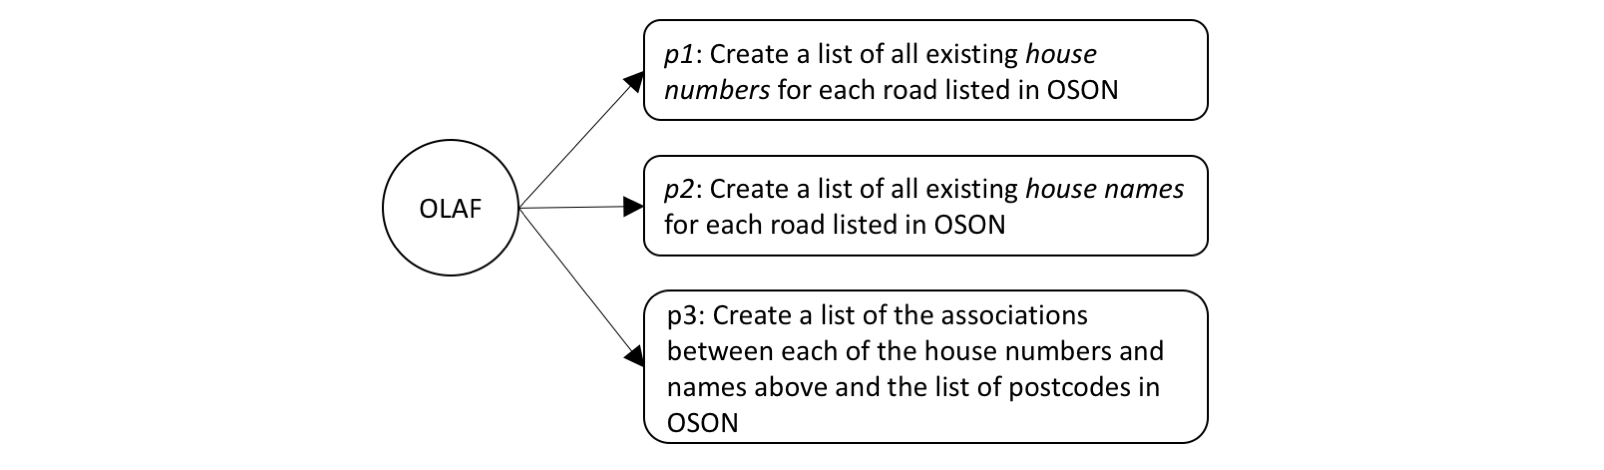
\includegraphics[width=1.0\textwidth]{problem-decomposition-1.png}
	\caption{A possible decomposition of the OLAF problem - First level}
	\label{fig:problem_decomposition_1}
\end{figure}

OSON "lists definitive place names, roads numbers and postcodes in Great Britain" and is instrumental to the work as it is the open dataset that is closer to the target, contentwise. In other words, OLAF can be seen as an augmentation of OSON, obtained by adding just one dimension to what can be already found in it, that is the list of house names and numbers associated to each of its roads and postcodes. 
    
Problems {\it p2}\footnote{Note that 98\% of UK addresses are characterised by a house number rather than a house name, so solving {\it p1} is substantially more relevant to achieve completeness in OLAF than {\it p2}.} and {\it p3} are not discussed further in this document. 

Problem {\it p1} can be further decomposed in four sub-problems as shown in figure \ref{fig:problem_decomposition_2}, thanks to the availability of additional open data sources and Land Registry's "Price Paid Data"\footnote{Land Registry is a non-ministerial UK Government department with the responsibility to register the ownership of land and property in England and Wales. See \url{https://www.gov.uk/government/collections/price-paid-data}.} ("LRPP") in particular. LRPP records every property ownership transfer in England and Wales since 1995, including their full addresses. It is just one of the several open data publications in the UK that include addresses, and the largest in size, hence particularly suitable to be used in the experiments.
    
\begin{figure}
	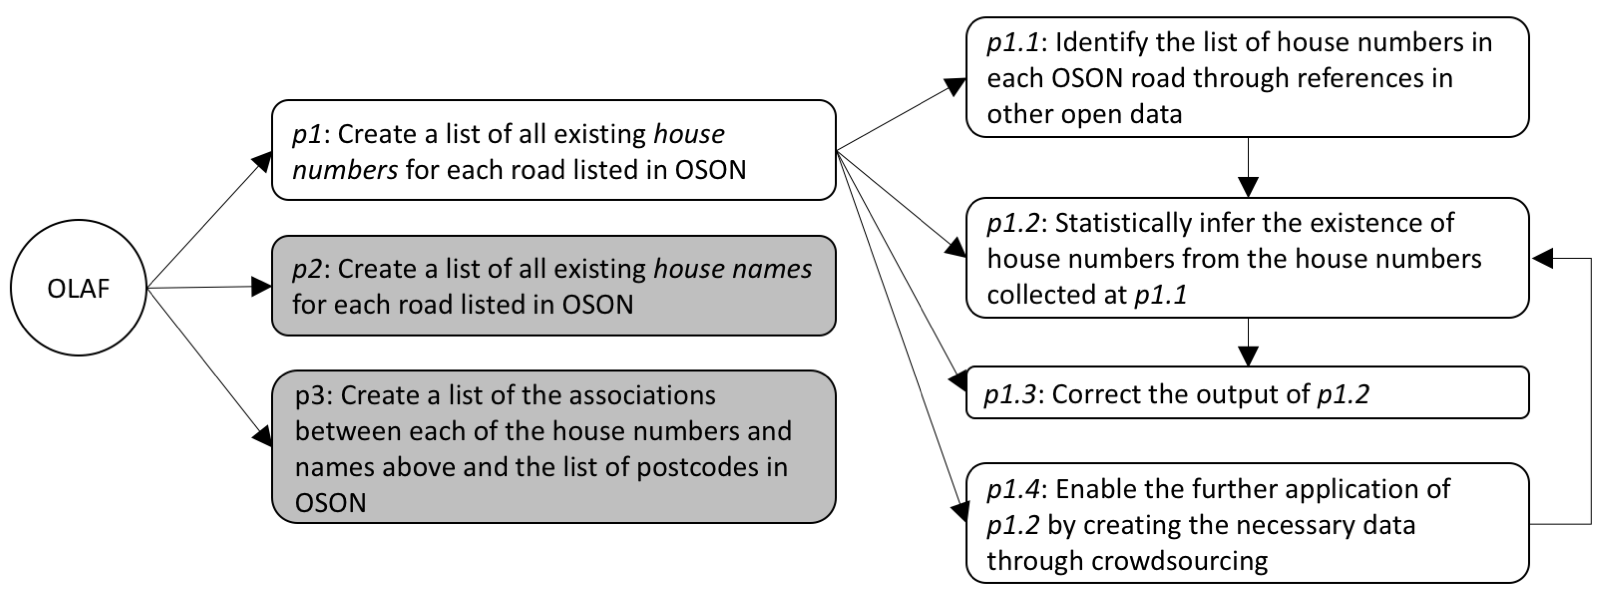
\includegraphics[width=1.0\textwidth]{problem-decomposition-2.png}
	\caption{A possible decomposition of the OLAF problem - First and second level}
	\label{fig:problem_decomposition_2}
\end{figure}

Problem {\it p1.3} is not discussed in this paper\footnote{Error in inferred house numbers is caused by three situations: (i) inferred house numbers for buildings that use house names instead (ii) inferred house numbers that in reality exist only in suffixed form (e.g. 7A instead of 7), and (iii) addresses that are simply missing, e.g. because a building was demolished. The volume of errors is considered not sufficient to compromise the use of inference. E.g. it can be calculated for (i) that the frequency of addresses identified by house names instead than house numbers is only 2\% of the total for the sampled geographic area. For (ii), the probability that a house number is used only in suffixed format is estimated to be 2.6\%, and that it is used {\it also} in suffixed format an additional 4.1\%. This is like saying that, out of 50 inferred house numbers, (i) 1 is in reality a house name, (ii) 2 are correct but are missing the suffixed variations and 1 is does not exist and should be replaced by its suffixed variations. Moreover, this is a worst case scenario, as the sample we used for the estimates is heavily urbanised.}.

\subsection{Creating a list of all existing house numbers for each road listed in OSON} 

Harvesting house numbers from LRPP and associating them to the OSON roads is possibly the simplest stage of the overall workflow, as the source datasets from OS and LR are good quality and well documented. Although the streets referenced in LRPP do not exactly match the ones in OSON (e.g. because of slightly different spelling, or being associated to localities rather than the main towns) it is possible to identify most of them without manual intervention and with a good degree of confidence.

\subsection{Inferring the existence of house numbers} 
\label{inference-algorithms} 

\textbf{House numbering convention} Inferring house numbers is strictly dependent on the numbering convention for the assignment of house numbers and names to buildings. Each culture developed its own over time. In the UK, buildings are typically numbered sequentially starting from 1, corresponding to the extremity of the road that is closest to the centre of the town. Odd numbers are on the left-hand side, as seen from the centre, while even number are on the right-hand side. House numbers can be suffixed by one or more letters: this is typical of larger buildings that at some point in time got divided into more smaller dwellings. 
        
\textbf{Inference algorithms} From knowing the numbering convention, inference can be used to create a large volume of missing house numbers from the observation of known house numbers. Algorithms \ref{algo:inference-numbers} and \ref{algo:inference-numbers-suffix} below have a very high probability to infer correctly the existence of house numbers\footnote{It should be considered, though, that centuries of house development and using the described numbering system loosely of course created many exceptions: e.g. there are buildings in the UK whose house number is zero, places where numbers were assigned consecutively on the same side of the street, and house numbers that are simply missing etc. Other available open data sources enable more complex algorithms, e.g. Ordnance Survey's "Open Maps - Local" includes summary shapes for the buildings in each street, hence enabling the detection of how many buildings are present and hint at which house numbers may be missing.}. 

\vspace{5mm}

\begin{algorithm}[H]
    \KwData{The list of known house numbers in a road}
    \KwResult{The list of inferred house numbers in the same road}
    \eIf{the list includes at least one even and one odd number}{
        infer all numbers between the lowest and the highest known numbers\;
    }{
        \If{the list includes at least two even or two odd numbers}{
            infer all even/odd numbers between the lowest and the highest numbers\;
        }
    }
    \caption{Inference of house numbers}
    \label{algo:inference-numbers}
\end{algorithm}

\vspace{5mm}

\begin{algorithm}[H]
    \KwData{The list of known house numbers with suffixes in a road}
    \KwResult{The list of inferred house numbers with suffixes in the same road}
    \For{each house number appearing in the list with at least two suffixes}{
        infer all suffixes between the lowest and the highest known suffix, in alphabetical order\;    
    }
    \caption{Inference of house number with suffixes}
    \label{algo:inference-numbers-suffix}
\end{algorithm}

\subsection{Enabling the application of the inference algorithms} 

It is evident from the specification of the algorithms that the inference of house numbers is enabled by one of the following two conditions: (a) the knowledge of two or more different house numbers in the same street and (b) the knowledge of two or more suffixes for the same number. The former has the highest potential to generate new house numbers. To infer the largest sets of numbers it is necessary to use as input the road's lowest and highest known house numbers\footnote{For simplicity, we did not consider (a) that it is also useful to know if the streets have both odd and even house numbers and (b) the case where one house number only is known for a street, for which we could assume 1 to be the lowest house number.}.

In order to evaluate the platform, it was deployed specifically to address this component of the overall problem and implement the workflow shown in Figure \ref{fig:workflow_2}.

\begin{figure}
	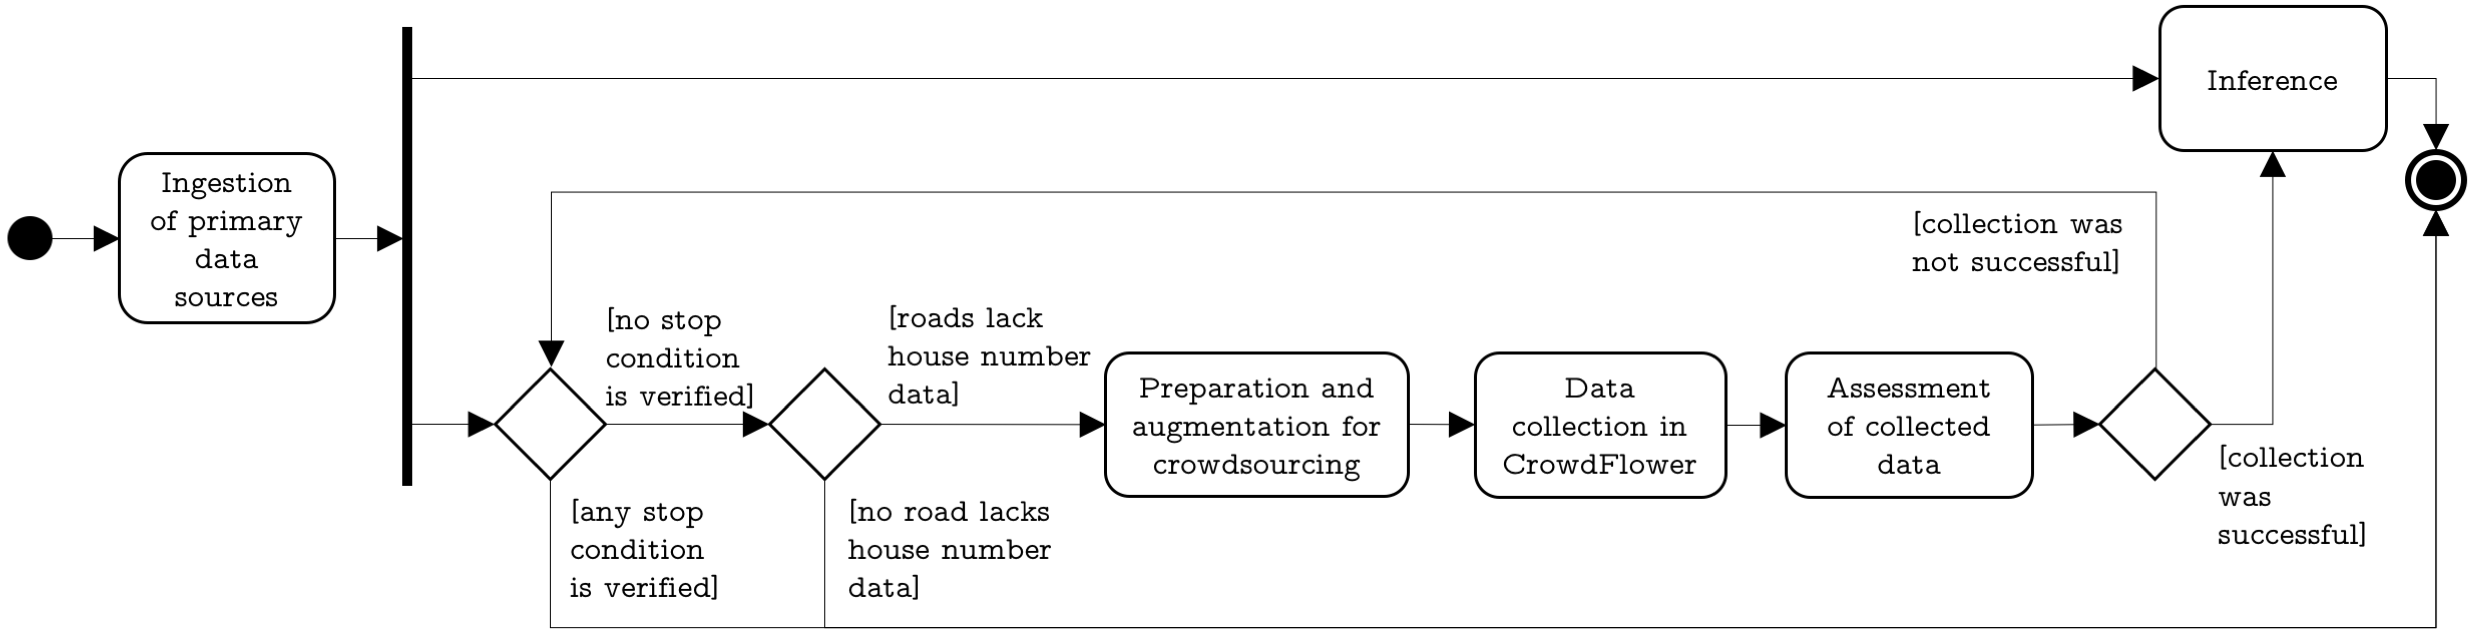
\includegraphics[width=1.0\textwidth]{workflow-2.png}
	\caption{UML process diagram of the OLAF-specific workflow developed for evaluation}
	\label{fig:workflow_2}
\end{figure}

The "stop conditions" referred to in the diagram are every condition not strictly related to the function of the system, e.g. the availability of budget. In other words, the workflow is iterated as long as budget is available, even if the aimed outcome is not achieved. 

Figure \ref{fig:workflow_1} shows in more detail which primary and derived datasets were used in each stage of the workflow. A new component is added to the picture, that is OS' "Open Roads"\footnote{See \url{https://www.ordnancesurvey.co.uk/business-and-government/products/os-open-roads.html}.} ("OSOR"). OSOR is used to calculate the geographical coordinates of the extremities of the roads where the lowest and the highest house numbers are more likely to be found. These are offered as "points of interest" to support the crowdworkers in their search. It is an example of how open data can be used not necessarily as a direct input into producing the output dataset, but to support the human participants in their function, too.

[CAN WE MAKE THIS PICTURE SMALLER?]

\begin{figure}
	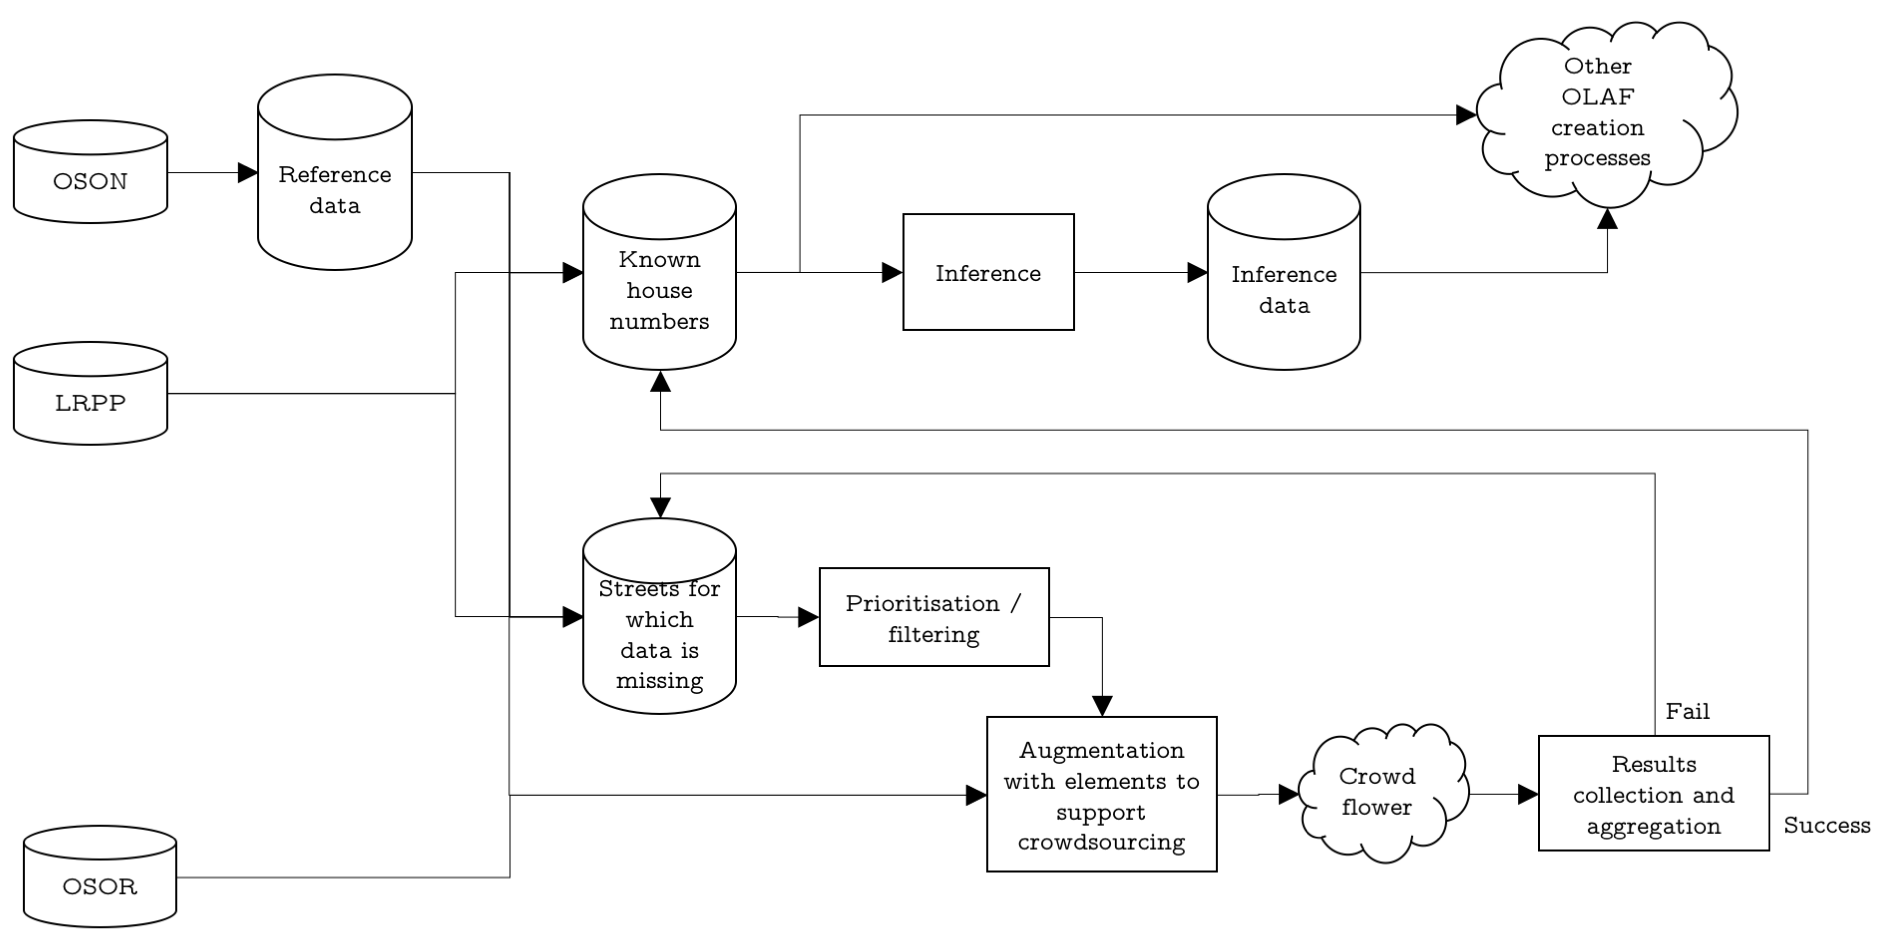
\includegraphics[width=1.0\textwidth]{workflow-1.png}
	\caption{Primary and derived datasets used to implement the workflow}
	\label{fig:workflow_1}
\end{figure}

\subsection{Crowdsourcing house numbers}

The crowdsourcing component of the platform can be configured to create the house numbers needed to enable inference. 

\textbf{Finding house numbers as a labelling exercise} Observing the imagery of a street to identify its lowest and highest house number is not conceptually different than crowdsourced annotation applications that extensively studied in literature, with the following exceptions:

\begin{itemize}
        
    \item For each item subject to annotation, two independent\footnote{One could argue that the two annotations are not truly independent, as the lowest house number is, by definition, lower than the highest house number. In practical terms, though, the task of surveying a street cannot leverage such mathematical relation. In other words, knowing what the highest house number is won't help the participant finding the lowest house number, as her finding is rather due to the observation of the topology of the street and the progression of nearby house numbers.} annotations rather than one are collected: the lowest and highest visible house numbers\footnote{It is not useful to as a participant to look for the lowest house number and another to look for the highest. By exploring the pictures, participants will naturally focus her research on the extremities of the road, where the relevant house numbers are, without knowing in advance which of the two she is finding first.}.
        
    \item The information subject to the annotation could be identified as existing, but the annotation may not be possible anyway\footnote{E.g. a participant may be able to identify the first house in a street, but vegetation may hide the number. There is also the possibility that the mapping provider coverage does not include the surveyed street. Moreover, unlike other countries, in the UK local authorities do not provide house number plates to the building owners, so this remains their responsibility. Building owners have the option not to affix any plate at all.}.
        
    \item The road to survey may be no buildings\footnote{Because of how the workflow was defined, crowdsourcing is used on streets of which there is little or no reference in LRPP over the last 20 years. This means that the road is likely rural and have few buildings.}.
        
\end{itemize}

The following is a description of the approach that was used for crowdsourcing addresses, that is common to all experimental conditions that were tested.

\subsubsection{Task model} \leavevmode \\ %% Why is this necessary to get a new line?

\textbf{Requester.} The Requester desires to gather the lowest and the highest house numbers that can be observed in a specified street, as they can be intelligibly identified by browsing pictures of the street. Alternatively, if no two house numbers are identifiable, the Requester needs being informed, too. Different streets have different degree of interest to the Requester, who is interested in prioritising the collection of the data for the higher interest streets in respect to the lower interest ones. The Requester requires the help of human agents to carry out the tasks, that we will call Workers in the following.

\textbf{Task.} Each HIT (Human Intelligence Task) consists of browsing the pictures of a street until achieving reasonable certainty of having identified the lowest and the highest house numbers or, alternatively, the lack thereof.

\textbf{Strategy.} 
The strategy relies on traditional crowdsourcing techniques for image labelling.

\textbf{Crowd $\rightarrow$ Worker.} Each Worker provides judgement on a task by browsing the pictures and declaring if she has found the lowest and the highest house numbers or none. Multiple Workers are asked to identify the house numbers for the same street. The resulting data is chosen through majority voting.

\textbf{Quality.} Quality is defined by a combination of (a) accuracy of the Workers in responding to tests questions, and (b) consensus in the data submitted through repeated surveys of the same road. Aggregation takes place accordingly as explained below.

\subsubsection{Workers quality}
    
Probing Workers using conventional test questions - e.g. where the correspondence of the Worker submissions is checked vs the same data collected by the research team as described in \cite{Kittur:2008gj} - would be a powerful tool to identify high vs low quality contributors, but is very expensive in OLAF's case. The task of surveying a street is not trivial, and early anecdotal evidence from early tests of the implementation showed many Workers leaving after performing no more than two or three surveys. To further damage the performance of the system, the ones who stayed longer started cheating, or showed a substantial drop in their performance. This suggested that spending a substantial part of the Worker's effort on test questions - e.g. making one out of three surveys a test - was not affordable.

Not using any kind of test question is unlikely to be successful, too, and it was explored in previous work such as \cite{DellaPenna:tf}. As an alternative, though, simple test questions can be set up on data that is already available, in a way that is similar to classic anti-spamming techniques like CAPTCHAs as described in \cite{Difallah:2012ty}. In OLAF's case the name of the street itself is used: Workers are asked to copy and paste or type the name of the street as part of their survey. Workers that do not achieve the target accuracy are excluded from further work.

\subsubsection{Results aggregation}

Repeated surveys of the same road are equivalent to the use of repeated judgement in conventional image labelling exercises. This practice is described extensively in literature and demonstrate that the results produced by a few expensive expert individuals are comparable to what emerges from involving multiple answers by crowds of non-expert Workers, e.g. in \cite{Snow:2008wo} and \cite{Sheng:2008gra}. As the answers are inevitably noisy, different Workers were asked to survey the same road, and their responses are aggregated to decide what is the most likely and truthful observation. 
        
Approaches to aggregation are an equally well studied subject, and a majority decision is a natural option (e.g. \cite{Le:2010ug}). The detailed parameters and process of how consensus is defined and calculated are tuned for better performance and address issues specific to the context (e.g. in \cite{Hirth:2011fh}). 

In the case of OLAF, consensus is measured by using Fleiss' kappa statistics for inter-annotator agreement, as described for example in \cite{Nowak:2010gt}. For those streets where the house numbers {\it were} found, a kappa of 60\% on at least 5 surveys is sufficient consensus (e.g. see \cite{Landis:1977kv}). For those streets where the house numbers were {\it not} found, a kappa of 80\% on at least 10 surveys is required instead, as it is more likely that unreliable Workers agree in reporting that.

The number of 5 and 10 judgements is chosen because they are respectively the minimum number of judgements where 60\% and 80\% kappa can be achieved without the need of an unanimous agreement (4 vs 1 for 60\% and 9 vs 1 for 80\%). 

Rounds of 5 surveys per road are performed until consensus is reached on both its lowest and highest house numbers. Because of the nature of the task, new surveys are performed even if consensus is reached already on either of the two numbers.  

\subsubsection{Recruitment}

We sourced all our Workers from CrowdFlower. For each experiment, we created one dedicated CrowdFlower job. We used identical settings for each experiment set, consisting of the following parameters:

\textbf{Geography} Limited to the top 10 contributor countries in CrowdFlower where English is an official or officially recognised language\footnote{See \url{https://success.crowdflower.com/hc/en-us/articles/202703345-Crowd-Demographics}, the identification of the countries was last repeated on 19 December 2015, before the running the experiments described in this paper. The list of countries is: Bangladesh, Canada, India, Malaysia, Netherlands, Pakistan, Philippines, Sri Lanka, United Kingdom and United States of America.}.

\textbf{Skills} We chose Workers from the default CrowdFlower performance category (formerly named "level 2"), that accounts for 29\% of the total population\footnote{See \url{https://success.crowdflower.com/hc/en-us/articles/202703345-Crowd-Demographics}, the calculation was done on 19 December 2015.}.

\textbf{Accuracy} As described in the previous section, as a test question Workers were asked to copy and paste or type the name of the street as part of their submission in each task. Being the question this simple, error was not accepted the requested accuracy was 99\%\footnote{CrowdFlower does not allow the Requester to set target accuracy to 100\%.}.

\textbf{Judgements} In groups of 5 per road, repeated until consensus is reached, by different Workers without repetition. Each Worker is allowed to contribute to as many tasks as possible.

\textbf{Behaviour} Each Worker was paid for 1 task, and 1 task is made of 1 street to survey.

\textbf{Reward / Time Limits} The reward was 0.20 US Dollars per task. Workers requiring less than 90 seconds per task were considered at high risk of being malicious and excluded to perform additional tasks. CrowdFlower imposes a time limit of 30 minutes maximum per task.

\subsection{Implementation}

[THIS IS STILL MISSING, WHAT DO I WANT TO WRITE MORE?]

(i) ingestion and preparation of the reference data\footnote{See the GitHub repository at \url{https://github.com/Digital-Contraptions-Imaginarium/OLAF-yr2_reference_data}.}, (ii) inference of house numbers where made possible from LRPP data\footnote{See the GitHub repository at \url{https://github.com/Digital-Contraptions-Imaginarium/OLAF-yr2_inference_data}.} and (iii) creation of the data for the crowdsourcing component and elaborating its results\footnote{See the GitHub repository at \url{https://github.com/Digital-Contraptions-Imaginarium/OLAF-yr2_lab}, {\it data-prep-scripts} and {\it analysis-scripts} folders respectively.}. 

[FIND SOME PLACE TO SAY WHY WE DON'T USE OPENSTREETMAP, BECAUSE SOMEONE WILL ASK. THE ANSWER IS THAT ITS LICENSING IS CONTROVERSIAL ACCORDING TO SOME: E.G. READ \cite{CentreforSpatialLawandPolicy:2014tx}]
    


\section{Results}

[SOMETHING ABOUT THE SAMPLE THE APPROACH WAS APPLIED TO, I HAD THIS BEFORE BUT WAS CUT OUT IN EDITING]

\begin{figure}
	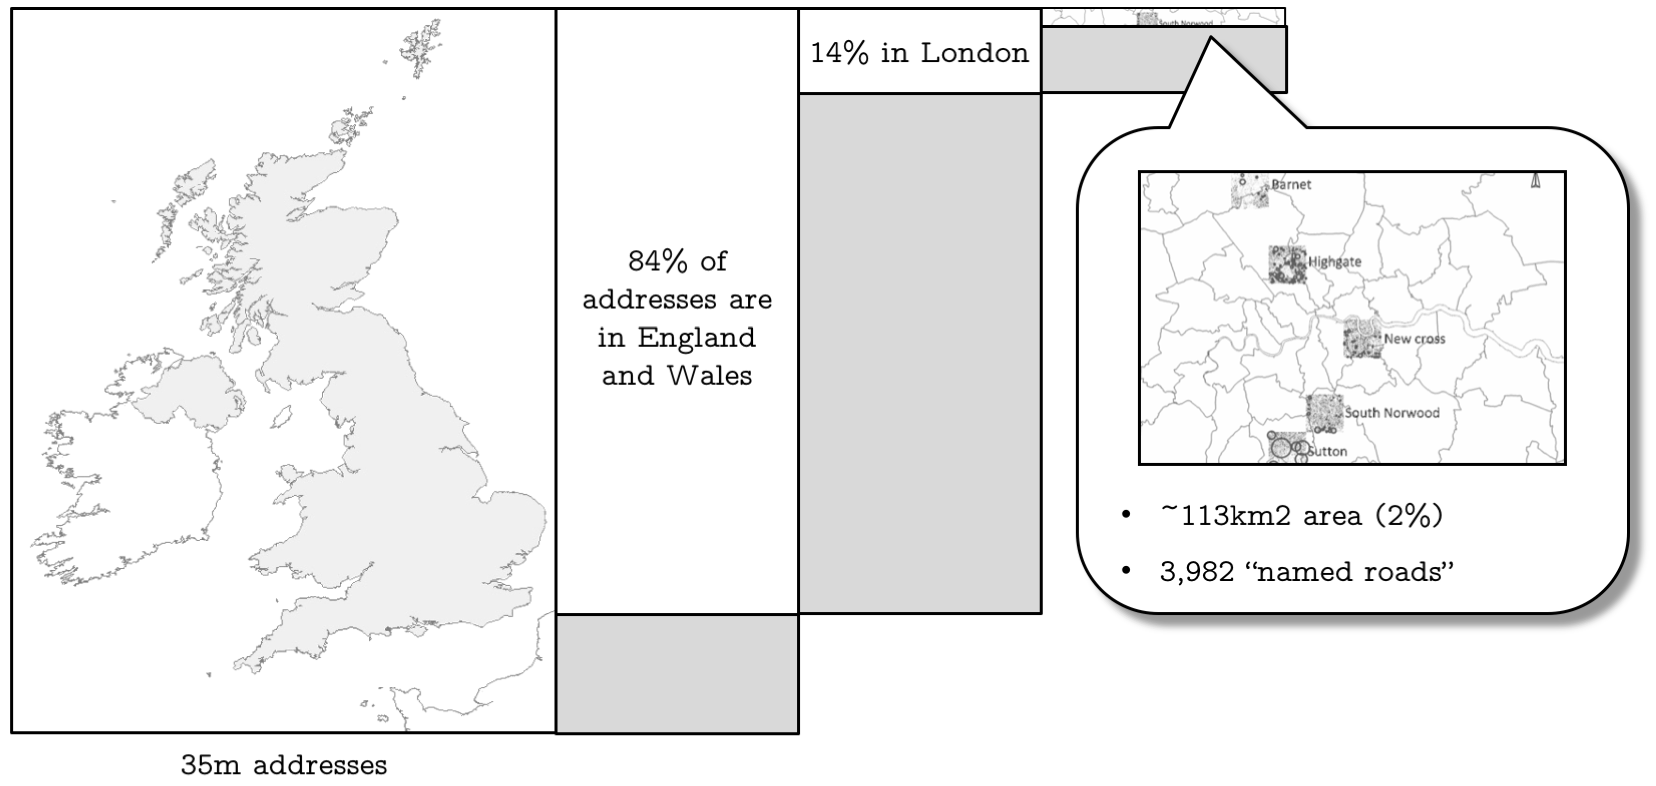
\includegraphics[width=1.0\textwidth]{scope.png}
	\caption{Scope for the evaluation}
	\label{fig:scope}
\end{figure}

\subsection{House number inference}

The implementation of the approach described in section \ref{crowdsourcing-olaf} showed that LRPP offers house numbers for 82\% of the streets in scope. The algorithms described in \ref{inference-algorithms} can be applied to the 74\% of roads, generating ~113k house numbers. 

\begin{figure}
	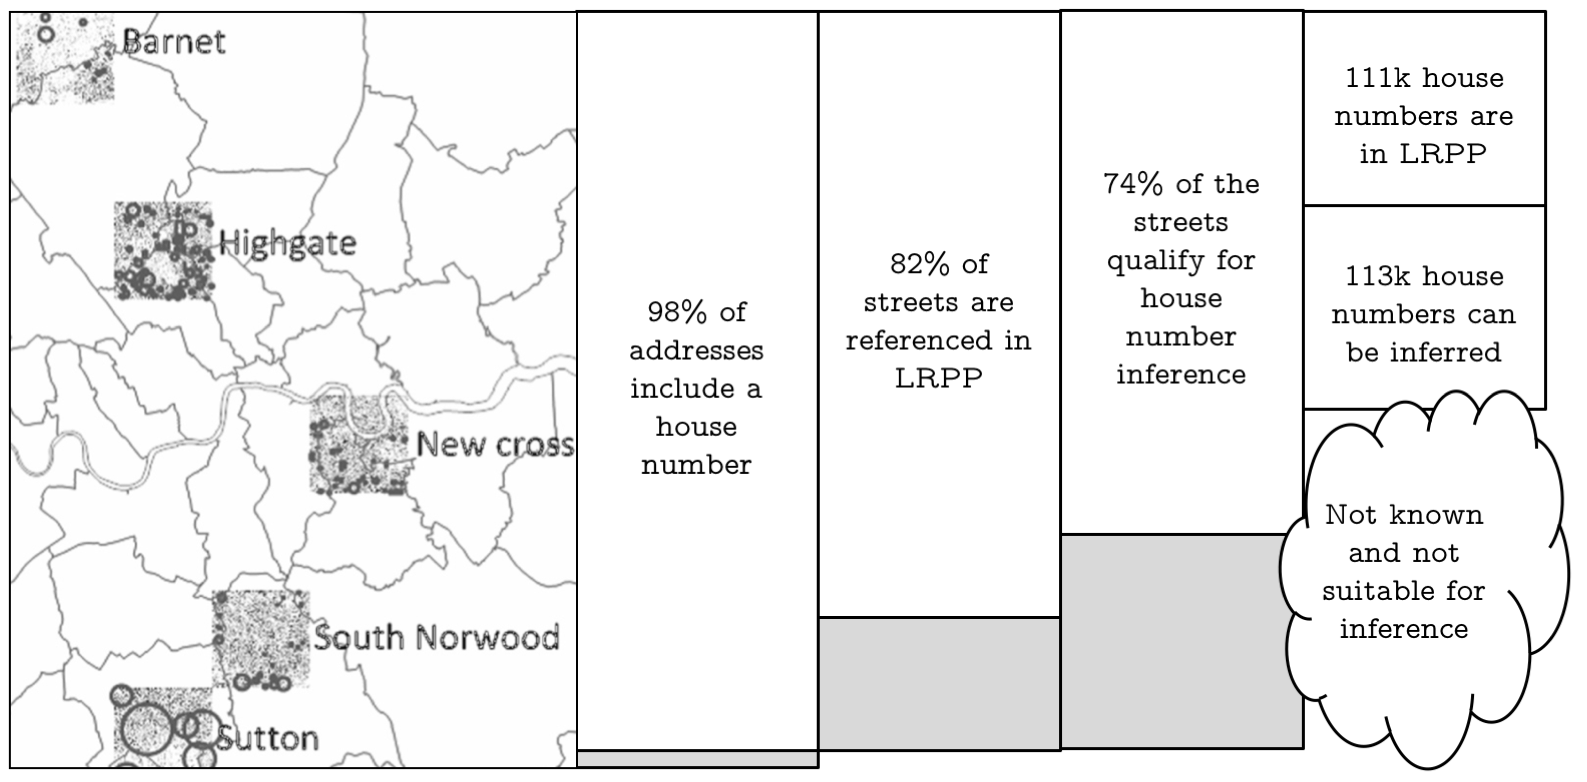
\includegraphics[width=1.0\textwidth]{inference-results.png}
	\caption{Results of inference application}
	\label{fig:results-inference}
\end{figure}

\subsection{BLAH}

The result of the experiment is summarised in tables \ref{table:distribution-of-workers} and \ref{table:judgements-summary} below. 

After three consecutive iterations and a total of 150 judgements per road by 80 Workers, the number of total duplicate judgements by reliable Workers was higher than the number of unique judgements, hence triggering the stop condition. 

18.75\% of Workers failed the simple test of copying the name of the road in the form, and were not considered trustworthy. 

Agreement could be reached on four streets only at the end of those three rounds. All roads were identified as not having house numbers.

Collection was reprised at a later point in time to attempt leveraging a different Worker base, through three additional rounds. The judgements of 41 additional Workers were collected, achieving consensus on three more roads. 

\begin{table}[]
\centering
\begin{tabular}{|l|c|c|l|l|}
\hline
                   & \multicolumn{1}{l|}{\begin{tabular}[c]{@{}l@{}}Tot. no. of \\ Workers\end{tabular}} & \multicolumn{1}{l|}{\begin{tabular}[c]{@{}l@{}}No. of new \\ Workers\end{tabular}} & \begin{tabular}[c]{@{}l@{}}No. of \\ reliable\\ Workers\end{tabular} & \begin{tabular}[c]{@{}l@{}}\% of \\ reliable \\ Workers\end{tabular} \\ \hline
First three rounds & 80                                                                                  & -                                                                                  & 65                                                                   & 81.25\%                                                              \\ \hline
All six rounds     & 121                                                                                 & 41                                                                                 & 97                                                                   & 80.16\%                                                              \\ \hline
\end{tabular}
\caption{Distribution of Workers across rounds}
\label{table:distribution-of-workers}
\end{table}



\begin{table}[]
\centering
\begin{tabular}{|l|l|l|l|}
\hline
                   & \begin{tabular}[c]{@{}l@{}}No. of \\ reliable\\ Workers\end{tabular} & \begin{tabular}[c]{@{}l@{}}No. of non-duplicate\\ judgements\end{tabular} & \begin{tabular}[c]{@{}l@{}}No. of roads\\ where consensus\\ was achieved\end{tabular} \\ \hline
First three rounds & 65                                                                   & 117                                                                       & 4                                                                                     \\ \hline
All six rounds     & 97                                                                   & 227                                                                       & 7                                                                                     \\ \hline
\end{tabular}
\caption{Judgement numbers and consensus summary}
\label{table:judgements-summary}
\end{table}

The graph below illustrates how Fleiss kappa variated...

\begin{figure}[!ht]
    \begin{floatrow}
        \ffigbox{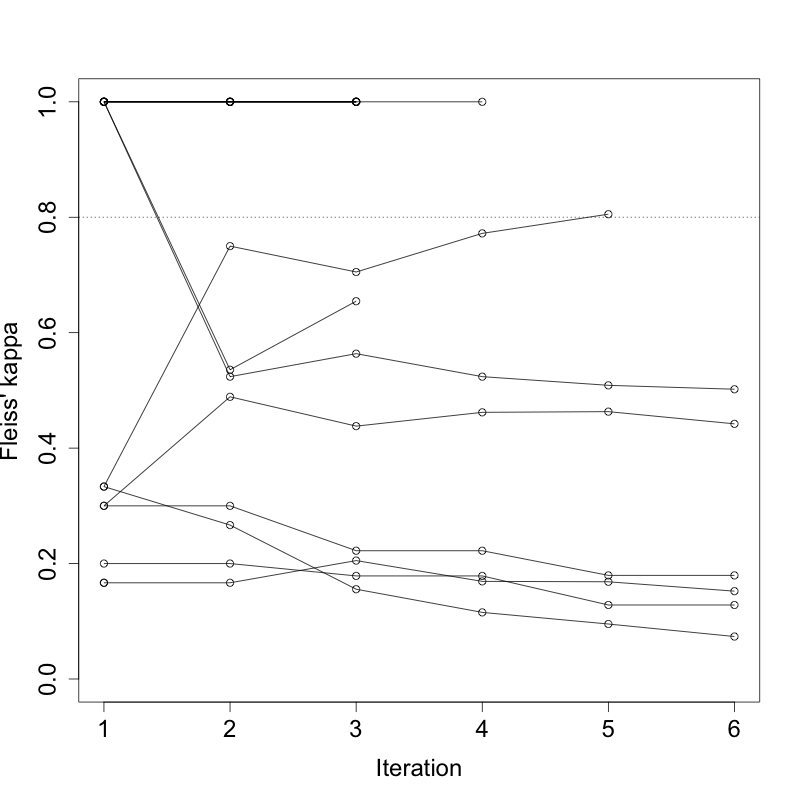
\includegraphics[width=0.5\textwidth]{results-lowest-not-found.png}}{\caption{Roads for which the house numbers were not found. Submissions for the lowest house number.}\label{fig:results-lowest-not-found}}
        \ffigbox{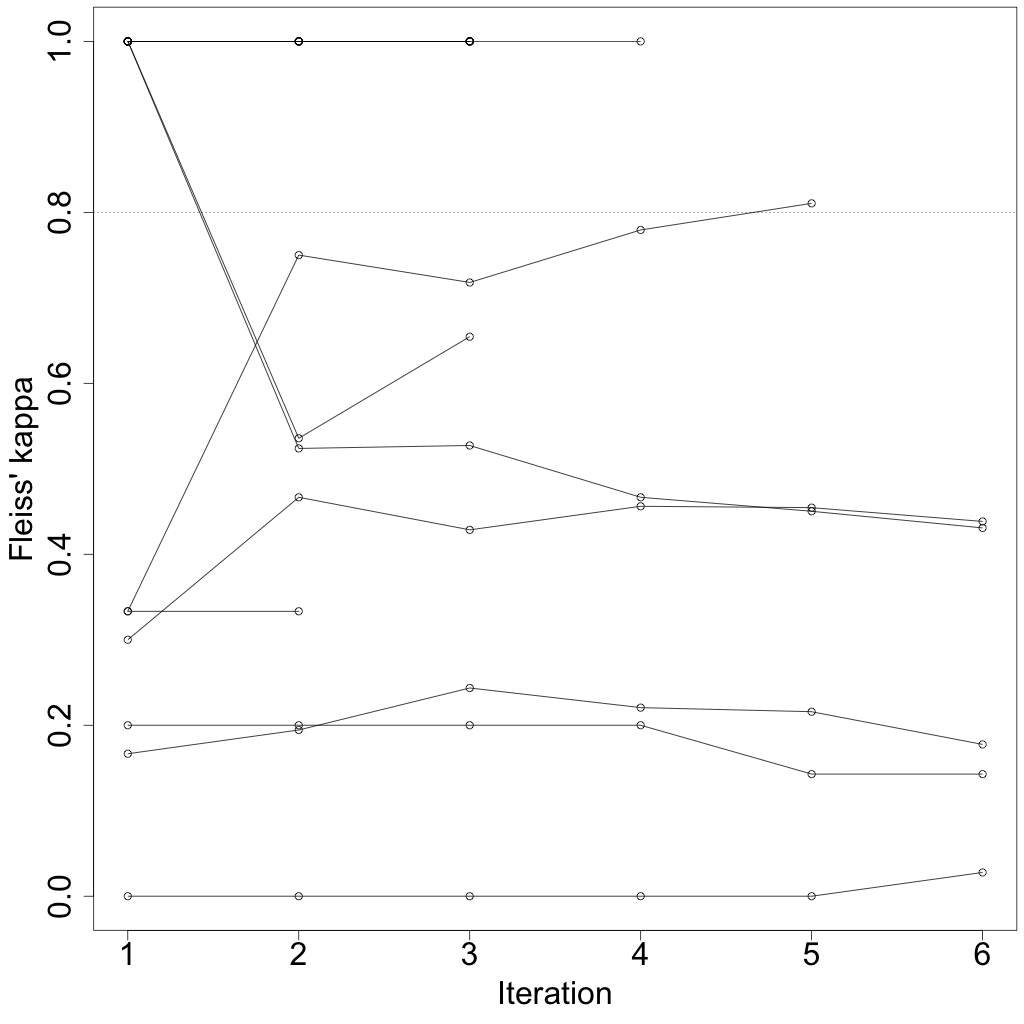
\includegraphics[width=0.5\textwidth]{results-highest-not-found.png}}{\caption{Roads for which the house numbers were not found. Submissions for the highest house number.}\label{fig:results-highest-not-found}}
   \end{floatrow}
\end{figure}
        
\begin{figure}[!ht]
    \begin{floatrow}
        \ffigbox{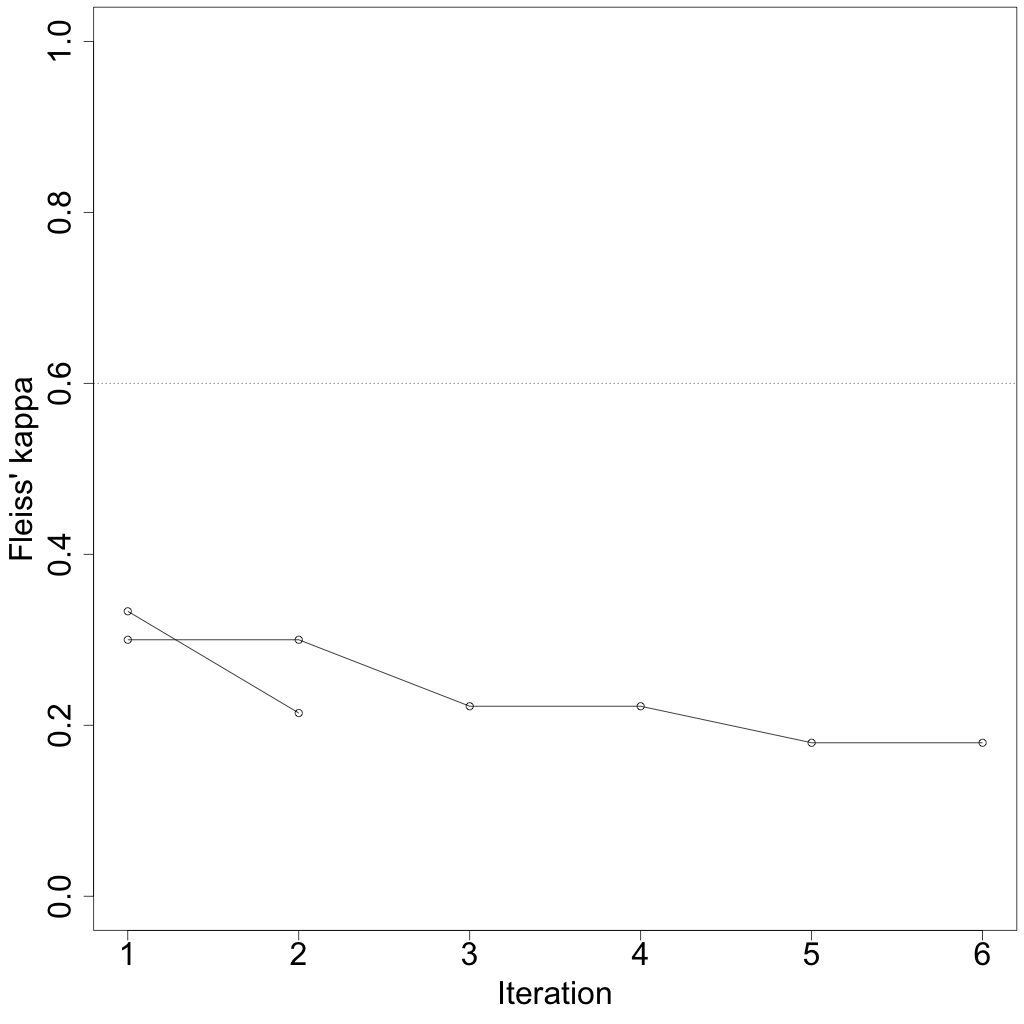
\includegraphics[width=0.5\textwidth]{results-lowest-found.png}}{\caption{Roads for which the house numbers were found. Submissions for the lowest house number.}\label{fig:results-lowest-found}}
        \ffigbox{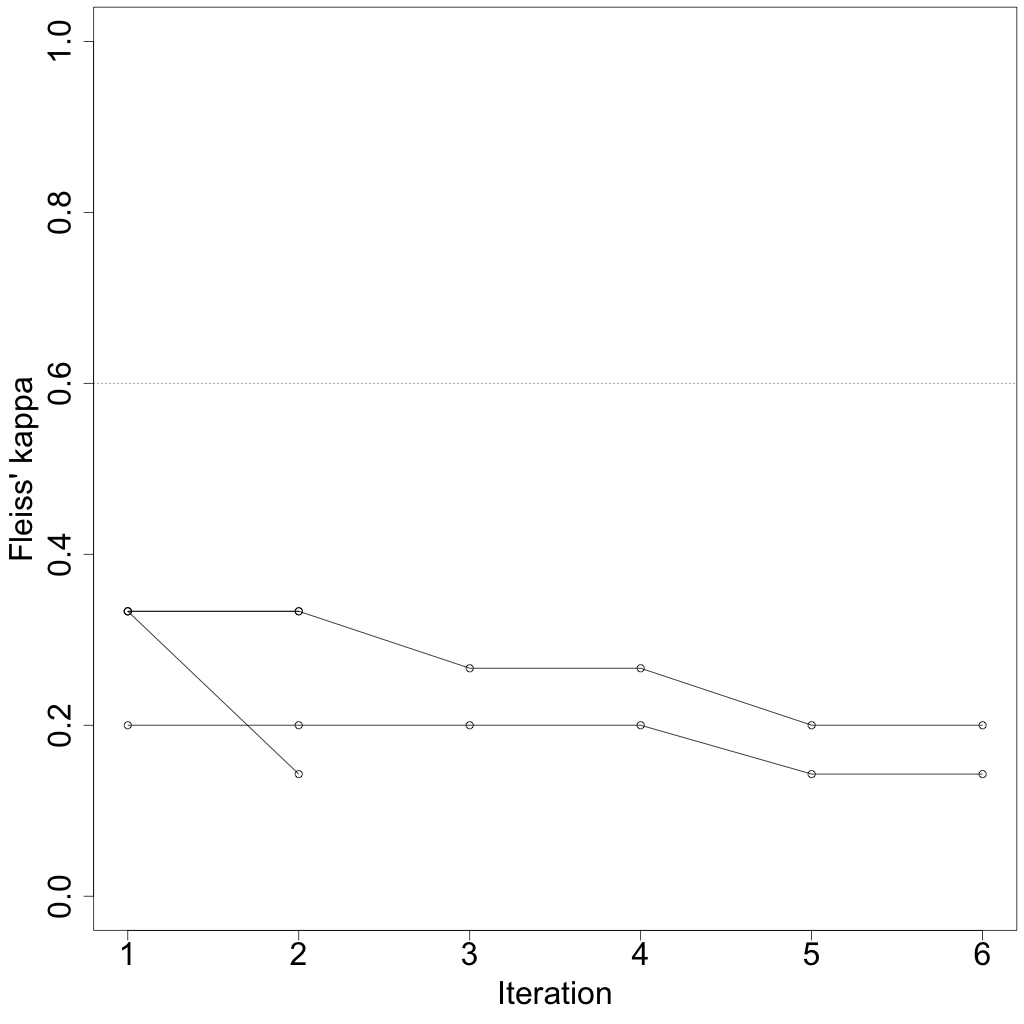
\includegraphics[width=0.5\textwidth]{results-highest-found.png}}{\caption{Roads for which the house numbers were found. Submissions for the highest house number.}\label{fig:results-highest-found}}
   \end{floatrow}
\end{figure}
        
\section{Discussion}

Because of its design, we believe our platform is virtually capable of achieving the maximum scalability and availability that is feasible within the limitations of the third party services we use as components, with CrowdFlower likely being the first potential bottleneck. We could not find documentation of CrowdFlower deployments relying on the involvement of large volume of users\footnote{Crowdflower documents some of its success stories at \url{http://www.crowdflower.com/success-stories}.} [DID ELENA SAY SHE HAD VISIBILITY OF A CROWDFLOWER USE CASE THAT GAVE INDICATION OF THEIR CURRENT CAPACITY?]. We expect though that the size of the full OLAF problem would be manageable by the platform, particularly considering that we would be still using it more as a complement to ingestion of primary data sources and computation rather than as the main channel to generate data.

Conversely, the decision to rely only on their native functionality, forced us to work around several of CrowdFlower's design characteristics that were not compatible with our crowdsourcing model. This forced us to implement the workflow in a way that was far from ideal and spend much more than necessary on Worker fees, e.g. because of Workers could not be prevented to judge the same road more than once. The detailed discussion of these issue is outside of the scope of this document, but the break-even point between relying on a crowdsourcing platform native functionality vs the cost and complexity of full customisation makes an interesting subject for further research.

As showed by the results, a much more pressing problem is the design of the crowdsourcing component. The model we used for evaluation in this paper failed to catalyse the contributors' agreement around results that are statistically credible. For sure, the complexity of the task and the open-ended nature of the survey activity were the root cause. Gottlieb {\it et al.} in \cite{Gottlieb:2012fh} expressed similar concern when exploring crowdsourcing to geolocate video.

Finally, even if we were successful, any discussion should still be filtered through a cost / benefit examination: what is a "reasonable cost" of producing one address with a target degree of confidence? Has a solution based on anything but VGI any opportunity to be cost effective? We may find that out the complexity of producing and maintaining an address file, to paraphrase the UK law, actually makes PAF's licensing price "reasonable".

\section{Conclusions}

We have presented WODA: a platform to integrate geospatial open data, computation and original human contribution to create original data, using human-machine hybrid workflows. To maximise the platform's scalability and availability, our design has relied as much as possible on the native features of mainstream SaaS services such as CrowdFlower and Google Maps. We have then implemented the platform to tackle components of one specific real life problem, that is the creation of OLAF: the list of all valid UK addresses. Where the conditions to enable computation were not verified, we deployed the platform to use paid microtask crowdsourcing to create the missing input data.

The evaluation of the platform has showed how critical the crowdsourcing component of the system is, particularly when it needs to support contributors in performing more complex activities than what is common in microtasking, such as surveying interactive imagery of locations. 

Moreover, our experience with CrowdFlower has also showed how third party services' native features may be intrinsically inconsistent with the needs of a workflow, de facto forcing the system designer to write ad hoc software that uses their API instead. This adds complexity and points of failure to the overall solution that could be avoided instead, and possibly compromises scalability and availability. 

Our plans for future work include exploring alternative configurations of pre-existing open data, computation and human contribution where the crowdsourcing component can be designed to achieve a higher degree of success. We also intend to share our work with the community of geospatial practitioners in London at one of their upcoming regular meetings, to gather feedback and ideas for further development.

Another interesting direction of research is to both (a) investigate how to re-design WODA to make the best use of the crowdsourcing provider's native functionality, and (b) work with them to implement those missing features and/or work around the limitations we identified during this work.


\textbf{Acknowledgements.} [WRITE THIS, NOTHING REVEALING IF THE REVIEW IS BLIND]

\documentclass{article}
\usepackage{url}
\begin{document}
\nocite{*}
\bibliography{main}
\bibliographystyle{splncs03}
\end{document}


\end{document}

